\documentclass[10pt,a4paper]{article}
\usepackage[margin=2.1cm]{geometry}
\usepackage[T1]{fontenc}
\usepackage[utf8]{inputenc}
\usepackage{lmodern}
\usepackage{amsmath,amssymb,amsthm}
\usepackage{graphicx}
\usepackage{microtype}
\usepackage[hidelinks]{hyperref}
\usepackage{url}
\Urlmuskip=0mu plus 1mu
\emergencystretch=2em

\newtheorem{theorem}{Theorem}
\newtheorem{lemma}[theorem]{Lemma}
\newtheorem*{remark}{Remark}
\newcommand{\R}{\mathbb{R}}
\newcommand{\Z}{\mathbb{Z}}

\title{Every non-5-colourable unit-distance graph in the plane\\ has at least 204 edges and at least 45 vertices}
\author{olivierFer3}
\date{November 2026 \quad (preprint, not yet reviewed by a human mathematician)}

\begin{document}
\maketitle

\begin{abstract}
We give a computer-assisted proof that every finite unit-distance graph in the Euclidean plane that
is not $5$-colourable has at least $204$ edges and at least $45$ vertices. The previous best bounds
were $182$ edges and $42$ vertices (de Grey--Parts). The proof combines the averaging argument of
Gwyn--Stavrianos with an explicit periodic $5$-colouring whose fifth colour sits on the midpoints of
one hexagon edge out of four, a computer-assisted upper bound
$p_5(c)\le 24616771/(5\cdot10^9)<1/203$ for its monochromatic unit-segment probability, obtained in
exact rational and ball arithmetic, and the bound $u(44)\le198$ derived from Proposition~12 of
\'Agoston--P\'alv\"olgyi.
\end{abstract}

\section{Statement and context}

A \emph{unit-distance graph} is a finite graph whose vertices are points of $\R^2$ and whose edges join
points at distance~$1$. Let $u(n)$ be the maximum number of edges of a unit-distance graph with $n$
vertices.

\begin{theorem}\label{thm:main}
Every finite unit-distance graph in $\R^2$ that is not $5$-colourable has at least $204$ edges and
at least $45$ vertices.
\end{theorem}

In the notation of \cite{dGP}, $e_6\ge204$ and $v_6\ge45$. The statement is unconditional: it says
nothing about the existence of such graphs. These quantities are finite if and only if
$\chi(\R^2)\ge6$. The inequality $\chi(\R^2)\ge6$ has been announced in an OpenAI preprint \cite{OAI},
which we have not checked; that preprint does not concern the bounds proved here. A simpler colouring (DISQP32 below) already gives $e_6\ge193$ and $v_6\ge44$.

\paragraph{Previous work.} Gwyn and Stavrianos \cite{GS} introduced $p_k(c)$, the probability that a
random unit segment is monochromatic for a $k$-colouring $c$ of the plane. They proved that a
non-$k$-colourable unit-distance graph has at least $1/p_k(c)$ edges \cite[Lemma~2.10]{GS}. With four
colours on regular hexagons, and a fifth colour on randomly translated disks
\cite[Lemma~2.23]{GS}, they obtained $e_6\ge180$. De Grey and Parts \cite{dGP} replaced the disks by
the rounded dodecagons of Croft's tiling, of density about $0.229365$ (Croft's ``tortoises''; see
\cite{KMOR} for the construction). They also corrected the rounding of the bounds, using
$e_k\ge\lceil1/p_{k-1}\rceil$ where \cite{GS} had rounded down, and they used the bounds on $u(n)$ of
\cite{AP}. This gave $e_5\ge99$, $v_5\ge28$, $e_6\ge182$ and $v_6\ge42$. Their values of $p_k$ were
computed by numerical integration (Mathematica) and were not certified. In the Polymath16 thread
\cite{PM16}, de Grey (commenting as \texttt{ag24ag24}) wrote on 28 June 2022 that he was ``hoping for a
more impressive value than 42 using good 5-tilings rather than their Lemma 6''. On 30 June 2022 he
reported that the hexagonal $5$-tiling he tried was worse and that ``something else is needed there --
I think probably an adaptation of the paper's Lemma 6 taking into account the existence of regions
that cannot contain a vertex of a mono edge''. We found no follow-up in the literature. The present construction is of
this kind: the fifth colour is not translated at random but placed at fixed positions relative to the
hexagons, on edge midpoints, and its shape is optimised. Related
but different problems include the numerical optimisation of periodic colourings
\cite{Mundinger} and partial proper colourings with voids \cite{Parts}.

\section{The colourings}

Fix rationals $R$ and $s\approx\sqrt3R$, and put $v_1=(3R/2,s/2)$, $v_2=(0,s)$, $\Lambda=\Z v_1+\Z v_2$,
$g_1=2v_1=(3R,s)$ and $g_2=2v_2=(0,2s)$. The colouring is periodic with period lattice
$G=\Z g_1+\Z g_2$, and its period cell $C$ has area $|C|=|\det(g_1,g_2)|$. The hexagon with centre
$c_{ij}=iv_1+jv_2$ receives colour $(i\bmod 2)+2(j\bmod 2)\in\{0,1,2,3\}$, as in \cite[Fig.~6]{GS}. Colour~$4$
is a region $E$ and its $G$-translates. $E$ is centred near the midpoint of the horizontal edge
shared by the hexagons $(0,0)$ and $(0,1)$, so the fifth colour covers one horizontal edge out of four.

\paragraph{ILEP256.} $R=283087619139/(5\cdot10^{11})$ and $s=196128855737/(2\cdot10^{11})$, so that
$|C|\approx3.33130$. The hexagons are slightly deformed. Their vertices are
$P_0(i,j)=c_{ij}+(R,0)+\delta_0[i\bmod2][j\bmod2]$ and $P_1(i,j)=c_{ij}+(R/2,s/2)+\delta_1[i\bmod2][j\bmod2]$,
with eight fixed rational displacements $|\delta|\le0.0068$. Hexagon $(i,j)$ is
$P_0(i,j)P_1(i,j)P_0(i{-}1,j{+}1)P_1(i{-}1,j)P_0(i{-}1,j)P_1(i,j{-}1)$, and these hexagons tile the plane.
The island $E$ is the polygon $W_0W_1\cdots W_{255}$ with
$W_k=m+\rho_k(\cos\psi_k,\sin\psi_k)$, $\psi_k=2\pi k/256$, rounded to $10^{-12}$. Here $m$ is the
midpoint of $P_1(0,0)P_0(-1,1)$, and $\rho$ is a piecewise-linear radial function with the symmetries
$\rho(\psi)=\rho(-\psi)=\rho(\pi-\psi)$. This formula only records how the island was generated: the certified object is the colouring
defined by the rational coordinates of the JSON files (see \emph{Exact definition} below). The island
has a nearly circular core of radius $0.43$--$0.48$
and four thin spikes ($\rho\approx0.58$) along the oblique edges. Its diameter is about $1.12$, and
pairs of points of colour~$4$, inside one island or in two islands, are counted. Exact
star-shapedness with respect to $m$ is checked: $\det(W_k-m,W_{k+1}-m)>0$ for all $k$, with total
angle $2\pi$.

\paragraph{DISQP32.} The hexagons are regular, up to the rounding of $s$, with $R=28360517/(5\cdot10^7)$.
$E$ is a rational $32$-gon of circumradius $0.48498$ centred at $(0,\,122773743/(2.5\cdot10^8))$.

\paragraph{Exact definition.} The certified colourings are the \emph{exact rational} colourings
defined by the files \texttt{ILEP256\_config.json} and \texttt{DISQP32\_config.json}. These files
list $g_1$, $g_2$ and a family of closed convex polygons $P_1,\dots,P_N$ with rational vertices, each
with a colour: 260 pieces for ILEP256 and 52 for DISQP32. The pieces are the hexagons minus the
fifth-colour regions, cut into convex pieces, together with convex sectors of $E$. They are
rational variants of the floating-point colourings found by optimisation. Because the argument
applies to any measurable periodic colouring, the bound concerns exactly these files. A point $x$
receives the colour of the piece of smallest index $i$ with $x\in P_i+G$. This rule is $G$-periodic and
Borel. Boundaries form a null set, so the rule does not affect $p_5$.
Figure~\ref{fig} shows ILEP256.

\begin{figure}[t]
\centering
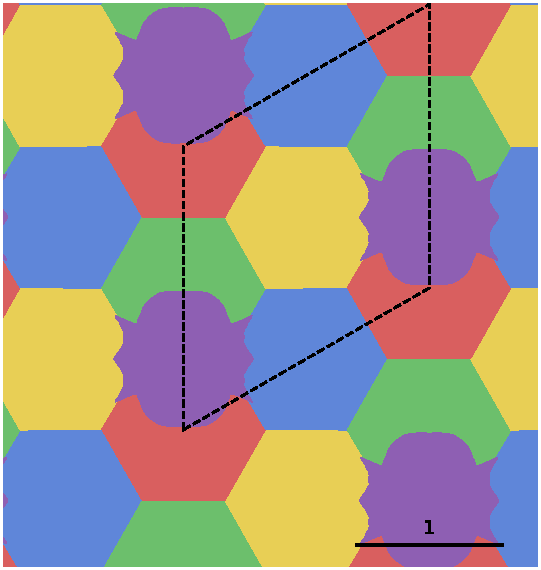
\includegraphics[width=0.98\textwidth]{fig_cellule.pdf}
\caption{Left: ILEP256 around one period cell (dashed parallelogram spanned by $g_1,g_2$). Red, blue, green,
yellow: colours $0$--$3$ on deformed hexagons. Purple: colour $4$ (the island). Right: zoom on the framed
island, with the boundaries of the convex pieces of the certified colouring. The bars have length $1$.}
\label{fig}
\end{figure}

\section{From \texorpdfstring{$p_5$}{p5} to edges and vertices}

For a $G$-periodic Borel colouring $c$, let $u(\theta)=(\cos\theta,\sin\theta)$ and
\[
p(c)=\frac{1}{2\pi|C|}\int_0^{2\pi}\bigl|\{x\in C:\ c(x)=c(x+u(\theta))\}\bigr|\,d\theta .
\]

\begin{lemma}[{\cite[Lemma~2.10]{GS}, periodic case}]\label{lem:gs}
If a finite unit-distance graph $H$ is not $k$-colourable and $c$ is a $G$-periodic Borel
$k$-colouring, then $|E(H)|\ge 1/p(c)$.
\end{lemma}
\begin{proof}
Draw $x$ uniformly in $\R^2/G$ and a rotation $\rho_\theta$ with $\theta$ uniform, and map $H$ by
$v\mapsto x+\rho_\theta v$. For each edge $vw$, the image of $v$ is uniform on $\R^2/G$ and
independent of the direction of $vw$, which is uniform. So the edge is monochromatic with
probability $p(c)$ (Fubini). The image of $H$ always has a monochromatic edge, so
$1\le\mathbb E[\#\text{mono}]=|E(H)|\,p(c)$.
\end{proof}

The same argument fits the framework of \cite{GS}, which uses Jordan measure. The set
$S=\{(x,\theta)\in C\times[0,2\pi]:c(x)=c(x+u(\theta))\}$ is Jordan-measurable in $\R^3$. Indeed, let
$Z$ be the union of the boundaries of the translates $P_i+g$. Two closed convex pieces with disjoint
interiors cannot meet the interior of each other, so $c$ is locally constant outside $Z$. Hence
$\partial S$ is contained in the union of $\partial(C\times[0,2\pi])$, of $\{(x,\theta):x\in Z\}$ and of
$\{(x,\theta):x+u(\theta)\in Z\}$, restricted to the compact set $\overline C\times[0,2\pi]$. Only
finitely many edges of $Z$ meet the bounded set $\overline C+\overline{B}(0,1)$. For each such edge
$z:[0,1]\to\R^2$, the corresponding parts of these two sets are the images of the two-dimensional set
$[0,1]\times[0,2\pi]$ under the Lipschitz maps $(t,\theta)\mapsto(z(t),\theta)$ and
$(t,\theta)\mapsto(z(t)-u(\theta),\theta)$. They therefore have three-dimensional measure zero, and so
does $\partial(C\times[0,2\pi])$. Thus $\partial S$ is a null set. By Lemma~\ref{lem:gs} and
Theorem~\ref{thm:cert} below, a non-$5$-colourable graph has more than $203.11$ edges, hence at least $204$.
DISQP32 gives at least $193$.

\paragraph{Vertices.} \'Agoston and P\'alv\"olgyi \cite[Prop.~12]{AP} state, for an \emph{extremal}
unit-distance graph $G$ with $n$ vertices and $m=u(n)$ edges, the inequality
$n^2-n\ge 4m-12n+24+\sum_v\binom{\deg v}{2}$. Its proof uses the construction of their Section~3:
unit circles around the vertices are cut into $2m$ arcs by the points of $G$. This requires every
vertex to have degree at least $3$, so that at least three points lie on each circle and every pair
of points is joined by at most two arcs. Extremality ensures that any two points at unit distance are
adjacent. We apply it only to an extremal graph $G$. If all degrees of $G$ are at least $3$, the
inequality holds. Otherwise, deleting a vertex of degree at most $2$ gives $u(n)\le u(n-1)+2$, as
noted in \cite[note~6, p.~12]{AP}. The sum is at least
$J(n,2m)=(n-r)\binom{q}{2}+r\binom{q+1}{2}$, where $2m=qn+r$ with $0\le r<n$. Let $P(n)$ be the
largest $m$ allowed by the inequality. Hence $u(n)\le B(n):=\max(P(n),B(n-1)+2)$. We start from the values and bounds of
\cite{AMP} for $n\le22$, and also use Schade's lemma $u(n)\le\lfloor n\,u(n-1)/(n-2)\rfloor$
\cite[Lemma~2]{AMP}, which is the better bound for $n\le32$. Recomputed in exact integer
arithmetic, this gives $u(43)\le192$ and $u(44)\le198$, in agreement with \cite[note~3]{dGP}. For
$n=44$ and $m=199$, the right-hand side equals $1894>1892=44^2-44$, so the bound is tight for the
method. Since $u$ is non-decreasing, a graph with at most $44$ vertices has at most $198<204$
edges. Therefore $v_6\ge45$, and DISQP32 gives $v_6\ge44$ because $u(43)\le192<193$.

\section{Certification of \texorpdfstring{$p_5$}{p5}}

\begin{theorem}\label{thm:cert}
For the exact colourings defined by the JSON files,
$p(\mathrm{DISQP32})\le 51864759/10^{10}<1/192$ and
$p(\mathrm{ILEP256})\le 24616771/(5\cdot10^9)<1/203$.
\end{theorem}

The floating-point values are $0.0051253$ and $0.0049197$. The final comparisons are exact:
$51864759\cdot192=9958033728<10^{10}$ and $24616771\cdot203=4997204513<5\cdot10^9$.

\paragraph{1. Exact tiling.} In rational arithmetic we check four facts. (i) Each piece is strictly
convex and counter-clockwise. This means all turns are positive \emph{and} the piece equals its
convex hull, a test that rejects star polygons. It holds for 52/52 and 260/260 pieces. (ii) The areas
of the pieces sum to $|C|$ exactly. (iii) Every pair $P_i$, $P_j+g$ with $(j,g)\ne(i,0)$ whose
bounding disks meet has an intersection of area~$0$. (iv) The list of translations is complete:
$|a|\,|C|\le|t|\,|g_2|$ for $t=ag_1+bg_2$, and similarly for $b$. Facts (ii) and (iii) imply that
the $G$-translates of the pieces partition the plane up to a null set.

\paragraph{2. Reduction to areas.} Let $A_{PQ}(u)=|P\cap(Q-u)|$. Using the symmetry
$p(\theta+\pi)=p(\theta)$, and no other symmetry, we get
\[ p(c)=\frac{1}{\pi|C|}\int_0^\pi\sum_{(P,Q)}A_{PQ}(u(\theta))\,d\theta, \]
where $P$ ranges over the pieces and $Q$ over the translates of pieces of the same colour.
Pairs of colour $4$ are included. A pair can contribute only if $\operatorname{dist}(0,Q-P)<1<
\max|{\rm vertex}(Q-P)|$, which leaves $394$ pairs for DISQP32 and $1804$ for ILEP256. On each box
of angles we also discard the pairs whose angular sector misses the box. The sector is enclosed
rigorously using ball arithmetic. Only translations with $|a|,|b|\le1$ can carry points at
distance $\le1$, so the enumeration with $|a|,|b|\le2$ is complete.

\paragraph{3. Bound on a box $I=[x_0\pi,x_1\pi]$.} (M1) By Brunn--Minkowski, the function $u\mapsto\sqrt{A_{PQ}(u)}$ (as a function of the translation
vector $u\in\R^2$, not of $\theta$) is concave on the support $\operatorname{int}(Q-P)$ of $A_{PQ}$.
Let $u_0$ be a rational point with $A_0=A_{PQ}(u_0)>0$ at which $A_{PQ}$ is differentiable, with
gradient $\nabla$; only this anchor point needs to be a point of differentiability. Put $d=u-u_0$
and $T=\sqrt{A_0}+\nabla\cdot d/(2\sqrt{A_0})$, the tangent of $\sqrt{A_{PQ}}$ at $u_0$. Concavity gives
$\sqrt{A_{PQ}(u)}\le T$ on the support, and $T\ge\sqrt{A_{PQ}(u)}\ge0$ there. Hence
$A_{PQ}(u)\le T^2=A_0+\nabla\cdot d+(\nabla\cdot d)^2/(4A_0)$. Outside the support, $A_{PQ}(u)=0\le T^2$.
So the bound holds for \emph{all} $u$. The gradient is exact: translating $Q-u_0$ by $-d$ moves only the edges $f$ of $Q-u_0$,
so $\nabla=-\sum_f n_f\,|f\cap P|$, with outer normals $n_f$. In the code, $P\cap(Q-u_0)$ is computed by
Sutherland--Hodgman clipping of $P$ by the half-planes of $Q-u_0$, and each edge of the intersection is
labelled as carried by $\partial P$ or by an edge of $Q-u_0$. Since the vectors (outer normal)$\times$(length)
of the edges of a closed polygon sum to zero, $\nabla=\sum_e n_e\,|e|$ over the edges $e$ of the
intersection labelled as carried by $\partial P$; this is the sum the code evaluates. Differentiability holds when no edge of $P$ is collinear with an edge of $Q-u_0$, which is
checked exactly. The right-hand side is a quadratic
polynomial in $(\cos\theta,\sin\theta)$ with rational coefficients, and its integral over $I$ is
evaluated from closed-form moments in ball arithmetic (Arb via python-flint, \cite{flint}). (M2) If
a rational rectangle $K$ contains the arc $u(I)$, then $A_{PQ}(u(\theta))\le|P\cap(Q\oplus(-K))|$ on
$I$. For each pair, either bound may be used; floating-point numbers only \emph{choose} $u_0$, the
bound and the boxes, so they never enter the validity. The box bounds are summed exactly. The total is
divided by $\pi|C|$ in ball arithmetic and rounded up. We use $256$ boxes for DISQP32 and $1024$ for
ILEP256, which take about $8$\,s and $155$\,s on a laptop.

\paragraph{Checks.} The written proofs of steps 1--3 were reviewed by a separate AI agent, including
the Sutherland--Hodgman clipping with edge labels used for the gradient. A second verifier, which does
not import the certifier, checks exactly, in Python \texttt{Fraction} arithmetic, the geometry of the
tiling (convexity, areas, disjointness, completeness of the translations), the list of contributing
pairs and the rational additions of the box bounds, including the final comparison with the lower
bound $\pi>314159265358979/10^{14}$. It does \emph{not} recertify in interval arithmetic each of the
$1280$ box bounds ($256+1024$): these rest on the Arb certifier alone. The second verifier also
recomputes every box integral in floating point (GEOS areas, explicit breakpoints, Gauss--Legendre),
and each certified box bound exceeds this integral, by at least $2.3\cdot10^{-9}$. The
Gauss--Legendre computations with 6 and 10 nodes agree to about $10^{-18}$. This agreement is a
numerical consistency check, not a rigorous bound on quadrature or GEOS errors. The rigorous upper
bounds rely exclusively on exact rational arithmetic and Arb interval enclosures. Independently of the
certificate, the same verifier recomputes $p(\mathrm{ILEP256})\approx0.0049197$. This shows that no
contribution is missing, but it is a consistency check, not a second proof.

\section{Limitations and remarks}

\begin{itemize}
\item \textbf{No human review yet.} The certificate, the proofs and the code have been checked only by
AI-assisted cross-checks, which may share blind spots. The proof rests on the inclusion principle of
Arb, which is standard and documented.
\item \textbf{Novelty.} To our knowledge $e_6\ge183$ and $v_6\ge43$ have not appeared before.
Our search covered arXiv, the tables of contents of Geombinatorics 2022--2026, the Polymath16 threads and
general web search. It is not exhaustive: we could not read the full text of recent Geombinatorics
issues, nor use Google Scholar.
\item \textbf{$\chi(\R^2)\ge6$} is not established independently here. Theorem~\ref{thm:main} holds in
any case.
\item \textbf{$v_6\ge46$} would require $p_5<1/205$. The floating-point value $p(\mathrm{ILEP256})\approx0.0049197$
does not allow it ($1/205\approx0.0048780$).
\end{itemize}

\begin{remark}[$v_5\ge29$]
From $e_5\ge99$ \cite{dGP} and $u(28)\le96$ \cite[Thm.~1(b)]{AMP}, it follows that every
non-$4$-colourable unit-distance graph has at least $29$ vertices. This remark uses only the published
bounds of \cite{dGP} and \cite{AMP}. As a secondary computation, not audited and not part of the
results of this note, the same certifier applied to the four-colour hexagon tiling with $D=1.133523$
gives $p_4\le101531397/10^{10}<1/98$, consistent with $e_5\ge99$.
\end{remark}

\paragraph{Use of AI.} The construction, the certification code, the proofs and this note were
produced with Claude Code (Anthropic). Additional AI agents and ChatGPT (OpenAI) performed
cross-checks: literature search, a reading of the arguments, execution of the verifiers and an
independent Monte Carlo estimate of $p_5$. These checks are AI-assisted and may share blind spots; no
human mathematician has reviewed this work yet.
Code and certificates: see the accompanying repository (\texttt{README.md}).

\begin{thebibliography}{9}\small
\bibitem{AMP} B.~Alexeev, D.~G.~Mixon, H.~Parshall, \emph{The Erd\H{o}s unit distance problem for small
point sets}, arXiv:2412.11914v2 (2025).
\bibitem{AP} P.~\'Agoston, D.~P\'alv\"olgyi, \emph{An improved constant factor for the unit distance
problem}, arXiv:2006.06285v3 (2021); Studia Sci.\ Math.\ Hungar.\ 59 (2022) 40--57.
\bibitem{dGP} A.~D.~N.~J.~de Grey, J.~Parts, \emph{On lower bounds of the order of $k$-chromatic unit
distance graphs}, arXiv:2303.14714v1 (2023); Geombinatorics 32(2) (2022), 72.
\bibitem{flint} FLINT/Arb documentation, \url{https://flintlib.org/doc/arb/index.html}; python-flint 0.9.0.
\bibitem{GS} H.~Gwyn, J.~Stavrianos, \emph{A finite graph approach to the probabilistic
Hadwiger--Nelson problem}, arXiv:2008.07987v1 (2020); Geombinatorics 32(1) (2022), 5.
\bibitem{KMOR} T.~Keleti, M.~Matolcsi, F.~M.~de Oliveira Filho, I.~Z.~Ruzsa, \emph{Better bounds for planar
sets avoiding unit distances}, Discrete Comput.\ Geom.\ 55 (2016) 642--661; arXiv:1501.00168v2.
\bibitem{Mundinger} K.~Mundinger, M.~Zimmer, A.~Kiem, C.~Spiegel, S.~Pokutta, \emph{Neural discovery in
mathematics: do machines dream of colored planes?}, arXiv:2501.18527v3 (ICML 2025).
\bibitem{OAI} OpenAI, \emph{The Euclidean plane is not five-colorable}, preprint (23 Sept.\ 2026),
\url{https://github.com/openai/math}.
\bibitem{Parts} J.~Parts, \emph{What percent of the plane can be properly 5- and 6-colored?},
arXiv:2010.12668; Geombinatorics 30(1).
\bibitem{PM16} D.~G.~Mixon (blog), \emph{Polymath16, seventeenth thread: declaring victory}, comments of
28 June 2022 (6:58 pm) and 30 June 2022 (12:22 am) by \texttt{ag24ag24},
\url{https://dustingmixon.wordpress.com/2021/02/01/polymath16-seventeenth-thread-declaring-victory/}.
\end{thebibliography}
\end{document}
